\documentclass[handout, notes=hide]{beamer}

\usepackage{amsmath}
\usepackage{yhmath}
\usepackage{eqnarray}
\usepackage{attrib}
\graphicspath{{./figures/}}
\DeclareGraphicsExtensions{.pdf,.jpeg,.png,.jpg}
\usepackage[export]{adjustbox}
\usepackage{framed}
\usepackage{tikz}
\usepackage{listings}
\usepackage{color}

\usetheme{Rochester}
\usecolortheme{beaver}

\setbeamertemplate{bibliography entry title}{}
\setbeamertemplate{bibliography entry location}{}
\setbeamertemplate{bibliography entry note}{}

\renewcommand{\thefootnote}{\fnsymbol{footnote}}
\newcommand{\prescite}[1]{\footnote{\cite{#1}}}
\newcommand{\prestext}[1]{\footnotetext{\cite{#1}}}
\newcommand{\emaillink}[1]{\href{mailto:#1}{\nolinkurl{#1}}}
\usepackage{perpage}
\MakePerPage{footnote}

\definecolor{shadecolor}{HTML}{E8F8FF}

\def\etal{{\it et al.}}
\def\etc{{\it etc.}}
\def\eg{{\it e.g.}}
\def\ie{{\it i.e.}}
\def\cf{{\it cf.}}
\def\qv{{\it q.v.}}
\def\qqv{{\it qq.v.}}
\def\st{s.t.\ }
\def\concat{\mathbin{|}}

\newtheorem{claimnum}{Claim}
\newtheorem{question}{Question}[section]

\newcommand\Wider[2][3em]{\makebox[\linewidth][c]{\begin{minipage}{\dimexpr\textwidth+#1\relax}\raggedright#2\end{minipage}}}
\newcolumntype{Y}{>{\centering\arraybackslash}X}
\newcommand{\comment}[1]{\marginnote{\textit{\textbf{\scriptsize{#1}}}}}
\newcolumntype{e}{@{\qquad}}



\definecolor{mygreen}{rgb}{0,0.6,0}
\definecolor{mygray}{rgb}{0.5,0.5,0.5}
\definecolor{mymauve}{rgb}{0.58,0,0.82}
 
%Customize a bit the look
\lstset{ %
	backgroundcolor=\color{white}, % choose the background color; you must add \usepackage{color} or \usepackage{xcolor}
	basicstyle=\fontsize{6pt}{6}, % the size of the fonts that are used for the code
	breakatwhitespace=false, % sets if automatic breaks should only happen at whitespace
	breaklines=true, % sets automatic line breaking
	captionpos=, % sets the caption-position to bottom
	commentstyle=\color{mygreen}, % comment style
	deletekeywords={...}, % if you want to delete keywords from the given language
	escapeinside={\%*}{*)}, % if you want to add LaTeX within your code
	extendedchars=true, % lets you use non-ASCII characters; for 8-bits encodings only, does not work with UTF-8
	frame=single, % adds a frame around the code
	keepspaces=true, % keeps spaces in text, useful for keeping indentation of code (possibly needs columns=flexible)
	keywordstyle=\color{blue}, % keyword style
	% language=Octave, % the language of the code
	morekeywords={*,...}, % if you want to add more keywords to the set
	numbers=left, % where to put the line-numbers; possible values are (none, left, right)
	numbersep=5pt, % how far the line-numbers are from the code
	numberstyle=\tiny\color{mygray}, % the style that is used for the line-numbers
	rulecolor=\color{black}, % if not set, the frame-color may be changed on line-breaks within not-black text (e.g. comments (green here))
	showspaces=false, % show spaces everywhere adding particular underscores; it overrides 'showstringspaces'
	showstringspaces=false, % underline spaces within strings only
	showtabs=false, % show tabs within strings adding particular underscores
	stepnumber=1, % the step between two line-numbers. If it's 1, each line will be numbered
	stringstyle=\color{mymauve}, % string literal style
	tabsize=2, % sets default tabsize to 2 spaces
	title=\lstname % show the filename of files included with \lstinputlisting; also try caption instead of title
}
%END of listing package%
 
\definecolor{darkgray}{rgb}{.4,.4,.4}
\definecolor{purple}{rgb}{0.65, 0.12, 0.82}
 
%define Javascript language
\lstdefinelanguage{JavaScript}{
	keywords={typeof, new, true, false, catch, function, return, null, catch, switch, var, if, in, while, do, else, case, break},
	keywordstyle=\color{blue}\bfseries,
	ndkeywords={class, export, boolean, throw, implements, import, this},
	ndkeywordstyle=\color{darkgray}\bfseries,
	identifierstyle=\color{black},
	sensitive=false,
	comment=[l]{//},
	morecomment=[s]{/*}{*/},
	commentstyle=\color{purple}\ttfamily,
	stringstyle=\color{red}\ttfamily,
	morestring=[b]',
	morestring=[b]"
}
 
\lstset{
	language=JavaScript,
	extendedchars=true,
	basicstyle=\fontsize{6pt}{6}\ttfamily,
	showstringspaces=false,
	showspaces=false,
	numbers=left,
	numberstyle=\fontsize{6pt}{6},
	numbersep=6pt,
	tabsize=2,
	breaklines=true,
	showtabs=false,
	captionpos=
}

%%%%%%%%%%%%%%%%%%%%%%%%%%%%%%%%%%%%%%%%%%%%%%%%%%%%%%%%%%%%%%%%%%%%%%%%%%%%%%%%%%

\begin{document}

\title{Cracking PwdHash: A Bruteforce Attack on Client-side Password Hashing}
\subtitle{Passwords 2016}
\author{David Llewellyn-Jones, Graham Rymer\\\vspace{0.5cm}\scriptsize\{David.Llewellyn-Jones, Graham.Rymer\}@cl.cam.ac.uk}
\institute{University of Cambridge}
\date{7th December 2016}

%%%%%%%%%%%%%%%%%%%%%%%%%%%%%%%%%%%%%%%%%

\renewcommand{\thefootnote}{\arabic{footnote}}

\frame{
\titlepage
\begin{tikzpicture}[remember picture,overlay]
\node[anchor=north east,yshift=-4pt,xshift=-4pt] at (current page.north east) {\includegraphics[height=0.9cm]{ucam-logo-colour}};
\end{tikzpicture}
}
\note{
\setlength{\parskip}{0.5em}
It begins.
}

\renewcommand{\thefootnote}{\fnsymbol{footnote}}

%%%%%%%%%%%%%%%%%%%%%%%%%%%%%%%%%%%%%%%%%

\begin{frame}
\frametitle{PwdHash}
\framesubtitle{What is PwdHash}
\setlength{\parskip}{0.5em}

\begin{columns}[T]
\begin{column}[T]{1.15\textwidth}
\vspace{-0.cm}
\hspace{-0.0cm}
\includegraphics[width=1.0\textwidth]{pwdhashsite}
\end{column}
\end{columns}

\end{frame}
\note{
\setlength{\parskip}{0.5em}
Graham

\begin{enumerate}
\item A password generating tool.
\item The user provides a site and a master password.
\item PwdHash generates a unique password for the site using a one-way hash function.
\end{enumerate}
}


%%%%%%%%%%%%%%%%%%%%%%%%%%%%%%%%%%%%%%%%%

\begin{frame}
\frametitle{PwdHash}
\framesubtitle{Where did PwdHash come from}
\setlength{\parskip}{0.5em}

\begin{columns}[T]
\begin{column}[T]{1.315\textwidth}
\vspace{-0.8cm}
\hspace{-0.8cm}
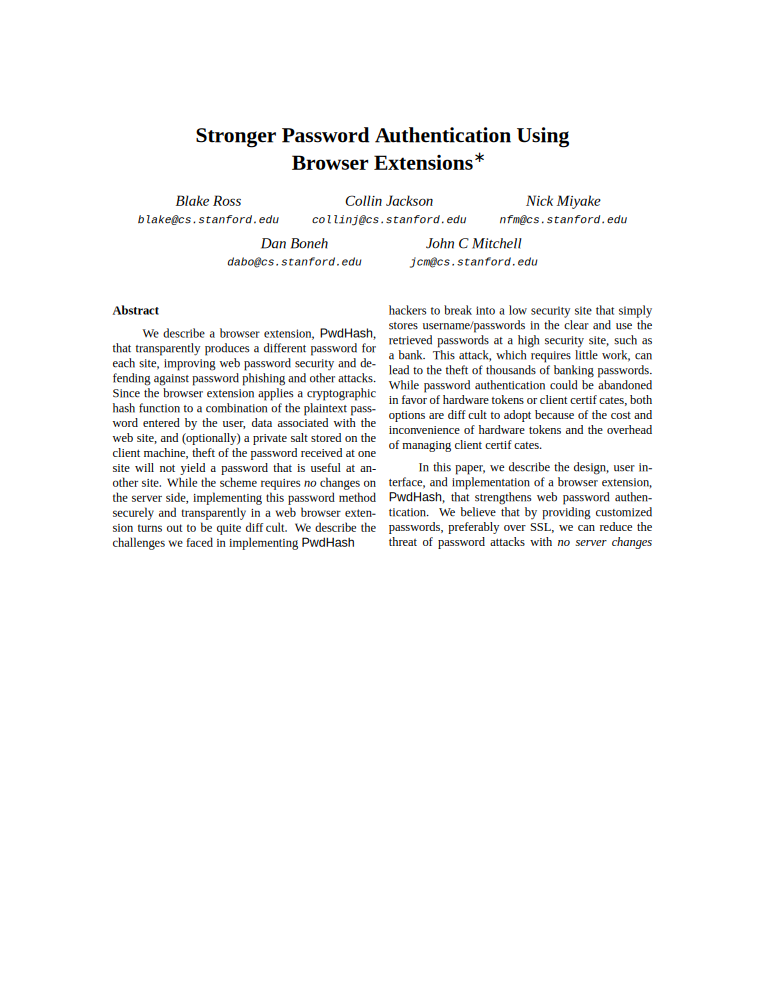
\includegraphics[width=1.0\textwidth]{ross2005}
\end{column}
\end{columns}

\end{frame}
\note{
\setlength{\parskip}{0.0em}
Graham

\begin{enumerate}
\item Published at USENIX 2005.
\item Blake Ross, Collin Jackson, Nick Mayake, Dan Boneh and John C Mitchell.
\item At the time at Stanford, but now in various places.
\begin{enumerate}
\item Blake co-founded Mozilla, until recently Director of Product at Facebook.
\item Jackson founded Apportable (cross-platform app dev).
\item Miyake was a student at the time.
\item Dan Boneh is Professor of Computer Science and Electrical Engineering at Stanford.
\item John C Mitchell is Professor of Computer Science and Electrical Engineering at Stanford.
\end{enumerate}
\end{enumerate}
}

%%%%%%%%%%%%%%%%%%%%%%%%%%%%%%%%%%%%%%%%%

\begin{frame}
\frametitle{Client-Side Hashing}
\framesubtitle{Not the first, or last}
\setlength{\parskip}{0.5em}

\begin{columns}[T]
\begin{column}[T]{0.6\textwidth}
\setlength{\parskip}{0.5em}
There are other examples of client-side hashing techniques
\begin{enumerate}
\item Passpet \\ \url{http://passpet.org}
\item PwdHash++ \\ IJAEST Vol 3, Issue 1, 2011
\item RndPhrase \\ \url{https://github.com/RndPhrase}
\end{enumerate}
\end{column}
\begin{column}[T]{0.4\textwidth}
\vspace{0.0em}
\includegraphics[width=1.0\textwidth]{android}
\end{column}
\end{columns}


\end{frame}
\note{
\setlength{\parskip}{0.0em}
David

\begin{enumerate}
\item Android app by Philipp Wolfer, updated April 2015 \url{https://play.google.com/store/apps/details?id=com.uploadedlobster.PwdHash}.
\item Firefox plugin updated February 2016 \url{https://addons.mozilla.org/en-US/firefox/addon/pwdhash/}
\item PassPet: SOUPS 2006, Ka-Ping Yee, Kragen Sitaker
\item PwdHash++: 2011, Venkata Prasad Reddy, Vedala Radha, Manik Jindal, International Journal of Advanced Engineering Sciences and Technologies
\item RndPhrase: Ronni Elken Lindsgaard, MSc, University of Copenhagen 
\end{enumerate}
}

%%%%%%%%%%%%%%%%%%%%%%%%%%%%%%%%%%%%%%%%%

\begin{frame}
\frametitle{PwdHash Operation}
\framesubtitle{How does it work?}
\setlength{\parskip}{0.5em}

\begin{columns}[T]
\begin{column}[T]{1.1\textwidth}
\vspace{0.0em}
\includegraphics[width=1.0\textwidth]{process01}
\end{column}
\end{columns}


\end{frame}
\note{
\setlength{\parskip}{0.5em}
Graham

High-level overview
}

%%%%%%%%%%%%%%%%%%%%%%%%%%%%%%%%%%%%%%%%%

\begin{frame}
\frametitle{PwdHash Operation}
\framesubtitle{How does it work?}
\setlength{\parskip}{0.5em}

\begin{columns}[T]
\begin{column}[T]{1.1\textwidth}
\vspace{0.0em}
\includegraphics[width=1.0\textwidth]{process02}
\end{column}
\end{columns}


\end{frame}
\note{
\setlength{\parskip}{0.5em}
Graham

High-level overview
}

%%%%%%%%%%%%%%%%%%%%%%%%%%%%%%%%%%%%%%%%%

\begin{frame}
\frametitle{PwdHash Operation}
\framesubtitle{How does it work?}
\setlength{\parskip}{0.5em}

\begin{columns}[T]
\begin{column}[T]{1.1\textwidth}
\vspace{0.0em}
\includegraphics[width=1.0\textwidth]{process03}
\end{column}
\end{columns}


\end{frame}
\note{
\setlength{\parskip}{0.5em}
Graham

High-level overview
}

%%%%%%%%%%%%%%%%%%%%%%%%%%%%%%%%%%%%%%%%%

\begin{frame}
\frametitle{PwdHash Operation}
\framesubtitle{How does it work?}
\setlength{\parskip}{0.5em}

\begin{columns}[T]
\begin{column}[T]{1.1\textwidth}
\vspace{0.0em}
\includegraphics[width=1.0\textwidth]{process04}
\end{column}
\end{columns}


\end{frame}
\note{
\setlength{\parskip}{0.5em}
Graham

High-level overview
}

%%%%%%%%%%%%%%%%%%%%%%%%%%%%%%%%%%%%%%%%%

\begin{frame}
\frametitle{Perceived Benefits}
\framesubtitle{What makes a good password?}
\setlength{\parskip}{0.5em}

\vspace{+2.0em}

\begin{columns}[T]
\begin{column}[T]{0.6\textwidth}
\setlength{\parskip}{0.5em}

Unique to each site

Contains complex mix of characters

Contains at least $n$ characters

Easy for the owner to remember, hard for anyone else to guess

\end{column}
\begin{column}[T]{0.4\textwidth}
\vspace{-3.0em}
\hspace{-7.0em}
\includegraphics[width=1.6\textwidth]{rockyou}
\end{column}
\end{columns}

\end{frame}
\note{
\setlength{\parskip}{0.5em}
Graham

The output from PwdHash appears to fulfil the requirements of what many people consider to be good password hygiene.

As a result, PwdHash passwords will achieve good `password strength' scores.
}

%%%%%%%%%%%%%%%%%%%%%%%%%%%%%%%%%%%%%%%%%

\begin{frame}
\frametitle{Other Benefits}
\framesubtitle{}
\setlength{\parskip}{0.5em}

\begin{columns}[T]
\begin{column}[T]{0.5\textwidth}
\setlength{\parskip}{0.5em}

No database of passwords

Can be used anywhere

Integrates into the browser

Protects against phishing

Can tailor the output to suit site restrictions

\end{column}
\begin{column}[T]{0.5\textwidth}
\includegraphics[width=1.0\textwidth]{plugin}
\end{column}
\end{columns}

\end{frame}
\note{
\setlength{\parskip}{0.5em}
Graham

There are also some other more practical benefits that PwdHash offers.
}

%%%%%%%%%%%%%%%%%%%%%%%%%%%%%%%%%%%%%%%%%

\begin{frame}
\frametitle{The Detail}
\framesubtitle{How does PwdHash work?}
\setlength{\parskip}{0.5em}

\begin{columns}[T]
\begin{column}[T]{1.0\textwidth}

\lstinputlisting[language=Javascript]{figures/pwdhashcode.js}

\end{column}
\end{columns}


\end{frame}
\note{
\setlength{\parskip}{-0.3em}
David

{\tiny
\begin{enumerate}
\item HMAC-MD5 is 16-types long.
\item Amounts to 22 characters in base64.
\item Passwords over 22 characters have A or zero byte repeatedly added, then no rotation.
\end{enumerate}

Important lines:
\begin{enumerate}
\item[5:] The output data is taken from base64 HMAC-MD5 of password and domain.
\item[6:] Final size will be two characters longer than input
\item[7:] Check whether any non-alphanumeric characters.
\item[13:] Four characters are removed that will be added back.
\item[18:] Add a capital letter.
\item[19:] Add a lowercase letter.
\item[20:] Add a number.
\item[21:] Add non-alphanumeric if necessary.
\item[23:] Remove non-alphanumerics if necessary.
\item[28:] Rotate the result.
\end{enumerate}
}%
}

%%%%%%%%%%%%%%%%%%%%%%%%%%%%%%%%%%%%%%%%%

\begin{frame}
\frametitle{Example Output}
\framesubtitle{}
\setlength{\parskip}{0.5em}

\begin{columns}[T]
\begin{column}[T]{1.0\textwidth}
\setlength{\parskip}{0.5em}

\renewcommand{\arraystretch}{1.5}
\begin{tabular}{l|p{2.5cm}|p{3.5cm}}
{\bf Site} & {\bf Password} & {\bf PwdHash password} \\ \hline
passwords2016.\colorbox{yellow}{rub.de} & passwords16 & 5CprBBsNjyvHQ \\
passwords2016.\colorbox{yellow}{rub.de} & passwords*16 & 3iL04G1ruj/rrK \\
www.\colorbox{yellow}{rub.de} & passwords*16 & 3iL04G1ruj/rrK \\
www.\colorbox{yellow}{linkedin.com} & passwords16 & HDOo1jM1emThY \\
www.\colorbox{yellow}{linkedin.com} & password012345 & QDHU4ZGr7dNfZOym \\
www.\colorbox{yellow}{linkedin.com} & 0123456789\newline 0123456789012 & aRnvjjBB5oV\newline 2f4b2ZA9EPAAAA \\
\end{tabular}
\end{column}
\end{columns}

\end{frame}
\note{
\setlength{\parskip}{0.5em}
David

Things to note:
\begin{enumerate}
\item Changing the password changes the hash. Adding a non-alphanumeric does the same for the output.
\item Changing the subdomain has no effect.
\item Chanding the domain changes the password.
\item The output increases in length with the password.
\item Go over 22 characters and it just appends `A's.
\end{enumerate}
}

%%%%%%%%%%%%%%%%%%%%%%%%%%%%%%%%%%%%%%%%%

\begin{frame}
\frametitle{The Problem}
\framesubtitle{Leaky password databases}
\setlength{\parskip}{0.5em}

\begin{columns}[T]
\begin{column}[T]{0.6\textwidth}
\setlength{\parskip}{0.5em}

HIBP contains 1.3 billion compromised accounts

@dumpmon identifies 46 significant database dumps per day

Discovered 1 million unique hashes in 12 months to May 2015

\end{column}
\begin{column}[T]{0.4\textwidth}
\vspace{0.0em}
\includegraphics[width=1.0\textwidth]{hibp}
\end{column}
\end{columns}


\end{frame}
\note{
\setlength{\parskip}{0.5em}
Graham

Saw similar results in David Jaeger's talk analysing publicly leaked credentials yesterday.
}

%%%%%%%%%%%%%%%%%%%%%%%%%%%%%%%%%%%%%%%%%

\begin{frame}
\frametitle{Salting and Hashing}
\framesubtitle{Modern best practice}
\setlength{\parskip}{0.55em}

\begin{columns}[T]
\begin{column}[T]{0.5\textwidth}
\setlength{\parskip}{0.5em}

Don't store the password in plaintext

Store a salted, hashed version

Use a slow hash function

$$
V = S \concat H(P \concat S)
$$

$V$ is the stored value,

$S$ a random salt,

$P$ the password,

$H$ is a one-way hash function

\end{column}
\begin{column}[T]{0.45\textwidth}
\includegraphics[width=1.0\textwidth]{boris}
\end{column}
\end{columns}


\end{frame}
\note{
\setlength{\parskip}{0.5em}
David

\begin{enumerate}
\item LinkedIn used unsalted SHA1.
\item Yahoo (late 2014, 500 million compromised accounts), mostly bcrypt hashed.
\end{enumerate}
}

%%%%%%%%%%%%%%%%%%%%%%%%%%%%%%%%%%%%%%%%%

\begin{frame}
\frametitle{Password Recovery}
\framesubtitle{Reversing salted hashes}
\setlength{\parskip}{0.5em}

\begin{columns}[T]
\begin{column}[T]{1.0\textwidth}
\setlength{\parskip}{0.5em}
Salting prevents use of rainbow tables

Hashes must be `reversed' by generating the hash and comparing

Recovery tools have responded by utilising GPUs

GPUs aren't necessarily as fast as CPUs, but are highly parallelisable

\end{column}
\end{columns}


\end{frame}
\note{
\setlength{\parskip}{0.5em}
David
}

%%%%%%%%%%%%%%%%%%%%%%%%%%%%%%%%%%%%%%%%%

\begin{frame}
\frametitle{Stats}
\framesubtitle{Password recovery is {\it fast}}
\setlength{\parskip}{0.5em}

\begin{columns}[T]
\begin{column}[T]{0.6\textwidth}
\setlength{\parskip}{0.5em}
Ruddick and Yan, 2016, analysed oclHashcat
\begin{itemize}
\item Radeon HD6870, 1120 processor streams at 900 MHz
\item SHA1, 1462 MH/s
\end{itemize}

Jeremy Gosney, Sagitta

\begin{itemize}
\item $8 \times$ Nvidia GTX Titan X
\item SHA1, 48.87 GH/s
\item bcrypt (cost 5) 133 KH/s.
\end{itemize}


\end{column}
\begin{column}[T]{0.4\textwidth}
\vspace{0.0em}
\includegraphics[width=1.0\textwidth]{hashcat}
\end{column}
\end{columns}


\end{frame}
\note{
\setlength{\parskip}{0.5em}
David

\begin{enumerate}
\item For SHA1, a 12-character base64 password space can be exhausted in just over 12 hours.
\end{enumerate}
}

%%%%%%%%%%%%%%%%%%%%%%%%%%%%%%%%%%%%%%%%%

\begin{frame}
\frametitle{Refining the Space}
\framesubtitle{Not just brute force}
\setlength{\parskip}{0.5em}

\begin{columns}[T]
\begin{column}[T]{1.0\textwidth}
\setlength{\parskip}{0.5em}

Scanning entire password space still not tractable

Use dictionaries and rules to refine

\begin{enumerate}
\item Masks
\item Combinator
\item Hybrid
\item Rule-based
\end{enumerate}

Generated PwdHash passwords aren't susceptible to these attacks

\end{column}
\end{columns}

\end{frame}
\note{
\setlength{\parskip}{0.5em}
Graham

\begin{enumerate}
\item Uniform distribution of characters.
\item Would require complete coverage of the password space.
\item The master password, however, is susceptible.
\end{enumerate}
}

%%%%%%%%%%%%%%%%%%%%%%%%%%%%%%%%%%%%%%%%%

\begin{frame}
\frametitle{PwdHash Attack}
\framesubtitle{Add the PwdHash hash into the hashcat process}
\setlength{\parskip}{0.5em}

\includegraphics[width=0.8\textwidth]{hashcat-usual}

\end{frame}
\note{
\setlength{\parskip}{0.5em}
David

This shows the standard recovery process for checking a single input value for a given leaked password.
}

%%%%%%%%%%%%%%%%%%%%%%%%%%%%%%%%%%%%%%%%%

\begin{frame}
\frametitle{PwdHash Attack}
\framesubtitle{Add the PwdHash hash into the hashcat process}
\setlength{\parskip}{0.5em}

\includegraphics[width=0.8\textwidth]{hashcat-pwdhash}

\end{frame}
\note{
\setlength{\parskip}{0.5em}
David

We introduce the PwdHash client-side step into the recovery process.

For PwdHash the salt $S_1$ is always empty.

The value $P_M$ is the password that would usually be sent to the server. For our approch it's just an intermediate value.
}


%%%%%%%%%%%%%%%%%%%%%%%%%%%%%%%%%%%%%%%%%

\begin{frame}
\frametitle{Hashcat Optimisations}
\framesubtitle{}
\setlength{\parskip}{0.5em}

\begin{columns}[T]
\begin{column}[T]{1.0\textwidth}
\setlength{\parskip}{0.5em}

Hashcat performs a variety of clever optimisations

Change only the first four bytes of the password

${\tt AAAA}\, {\tt pass}\, {\tt word}$ \\
$\underbrace{{\tt\vphantom{p}AAAB}}_{w[0]}\underbrace{{\tt\vphantom{p}pass}}_{w[1]}\underbrace{{\tt\vphantom{p}word}}_{w[2]}$

MD5 meet-in-the-middle-attack, see Jens Steube's Passwords13 talk: \url{https://hashcat.net/events/p13/}

SHA1 optimisation
\begin{enumerate}
\item 512-bit input extended to 2560-bits using XOR and ROL
\item Precompute inputs without first four bytes
\end{enumerate}

\end{column}
\end{columns}


\end{frame}
\note{
\setlength{\parskip}{0.5em}
David

Unfortunately it's not quite this simple, because of the hashcat optimisations.
}

%%%%%%%%%%%%%%%%%%%%%%%%%%%%%%%%%%%%%%%%%

\begin{frame}
\frametitle{PwdHash Attack}
\framesubtitle{Add the PwdHash hash into the hashcat process}
\setlength{\parskip}{0.5em}

\includegraphics[width=1.0\textwidth]{process-orig}

\end{frame}
\note{
\setlength{\parskip}{0.5em}
David

This is the usual hashcat approach with the base pre-computation stage as an optimisation.

The pre-computation step assumes only the first four characters will change.
}

%%%%%%%%%%%%%%%%%%%%%%%%%%%%%%%%%%%%%%%%%

\begin{frame}
\frametitle{PwdHash Attack}
\framesubtitle{A problem}
\setlength{\parskip}{0.5em}

\begin{columns}[T]
\begin{column}[T]{1.0\textwidth}
\setlength{\parskip}{0.5em}

The PwdHash step messes up the optimisation

${\tt AAAA}\, {\tt pass}\, {\tt word} \quad \longmapsto \quad {\tt KZvm}\, {\tt M4fs}\, {\tt sCZ6}\, {\tt 96\quad}$ \\
$\underbrace{{\tt\vphantom{p}AAAB}}_{w[0]}\underbrace{{\tt\vphantom{p}pass}}_{w[1]}\underbrace{{\tt\vphantom{p}word}}_{w[2]} \quad \longmapsto \quad \underbrace{{\tt\vphantom{p}9us7}}_{w[0]}\underbrace{{\tt\vphantom{p}NzXw}}_{w[1]}\underbrace{{\tt\vphantom{p}LaCJ}}_{w[2]}\underbrace{{\tt\vphantom{p}Zw\quad }}_{w[3]}$

\end{column}
\end{columns}


\end{frame}
\note{
\setlength{\parskip}{0.5em}
David

Unfortunately this assumption no longer applies for us.

A small change in the input value results in all characters changing.

Consequently we can't perform the same base pre-computation optimisation..
}

%%%%%%%%%%%%%%%%%%%%%%%%%%%%%%%%%%%%%%%%%

\begin{frame}
\frametitle{PwdHash Attack}
\framesubtitle{Add the PwdHash hash into the hashcat process}
\setlength{\parskip}{0.5em}

\includegraphics[width=1.0\textwidth]{process-orig}

\end{frame}
\note{
\setlength{\parskip}{0.5em}
David
}

%%%%%%%%%%%%%%%%%%%%%%%%%%%%%%%%%%%%%%%%%

\begin{frame}
\frametitle{PwdHash Attack}
\framesubtitle{Add the PwdHash hash into the hashcat process}
\setlength{\parskip}{0.5em}

\includegraphics[width=1.0\textwidth]{process-mangle}

\end{frame}
\note{
\setlength{\parskip}{0.5em}
David

The pre-computation could be used for multiple passwords. Now we must do it for every password.

So we move some of the pre-computation into the main loop.

You might expect that this would have a performance hit, which we'll look at later.
}

%%%%%%%%%%%%%%%%%%%%%%%%%%%%%%%%%%%%%%%%%

\begin{frame}
\frametitle{Results}
\framesubtitle{Summary of leaked hash databases tested}
\setlength{\parskip}{0.5em}

\begin{columns}[T]
\begin{column}[T]{1.0\textwidth}
\setlength{\parskip}{0.5em}

\fontsize{9pt}{14}\selectfont

\begin{tabular}{l|p{2.0cm}|p{2.0cm}|p{2.2cm}}
	{\bf Domain} & Stratfor.com & Rootkit.com  & Linkedin.com \\ \hline
	{\bf Year of leak}   & 2011         & 2011         & 2012 \\
	{\bf Hashes} & 822 657      & 58 677       & 2936840/ 6458020 \\
	{\bf Type}   & Unsalted MD5 & Unsalted MD5 & Unsalted SHA1 \\
	{\bf Attribution} & ``Anonymous'' & ``Anonymous'' & Unknown \\
	{\bf Previous best effort} & 93\% & 95\% & 77\% \\
	{\bf Cracking speed} & 42008.5 kH/s & 42193.8 kH/s & 39762.2 kH/s \\
	{\bf } & (11.40ms/H) & (11.35ms/H) & (14.88ms/H) \\
	{\bf Cracking time} & 27s & 27s & 28s \\
	{\bf Passwords recovered} & 1 & 3 & 75 \\
\end{tabular}

\end{column}
\end{columns}


\end{frame}
\note{
\setlength{\parskip}{0.5em}
Graham
}

%%%%%%%%%%%%%%%%%%%%%%%%%%%%%%%%%%%%%%%%%

\begin{frame}
\frametitle{Benchmarks}
\framesubtitle{Testing rig}
\setlength{\parskip}{0.5em}

\begin{columns}[T]
\begin{column}[T]{0.7\textwidth}
\setlength{\parskip}{0.5em}

Amazon EC2 g2.2xlarge instance

Eight Intel Xeon E5-2670 vCPUs - 2.60GHz

NVIDIA GRID K520 - 800 MHz

Two GPUs with 1536 CUDA cores (3072 total)

4GB of graphics memory and 8 GB main RAM

Costs \$0.65 per hour

\end{column}
\begin{column}[T]{0.3\textwidth}
\vspace{0.0em}
\includegraphics[width=1.0\textwidth]{k520}
\end{column}
\end{columns}

\end{frame}
\note{
\setlength{\parskip}{0.5em}
Graham

Not the best machine or graphics card.

However, cheaper than buying a machine from scratch.
}

%%%%%%%%%%%%%%%%%%%%%%%%%%%%%%%%%%%%%%%%%

\begin{frame}
\frametitle{Benchmarks}
\framesubtitle{How does this impact performance?}
\setlength{\parskip}{0.5em}

\includegraphics[width=1.0\textwidth]{benchmarks}

\end{frame}
\note{
\setlength{\parskip}{0.5em}
David

\begin{tabular}{p{3.7cm}|p{2.6cm}|p{3.0cm}}
	{\bf Hash type} & {\bf Speed (MH/s)} & {\bf Overhead (factor)} \\ \hline
	MD5 & 2316.7 & 1.0 \\
	MD5 PwdHash & 2410.7 & 0.961 \\
	SHA1 & 616.9 & 1.0 \\
	SHA1 PwdHash & 645.1 & 0.956 \\
	HMAC-MD5 & 780.3 & 1.0 \\
	HMAC-MD5 PwdHash & 76.9527 & 10.140 \\
	Stratfor.com MD5 & 42.0085 & n/a \\
	Rootkit.com MD5 & 42.1938 & n/a \\
	Linkedin.com SHA1 & 39.7622 & n/a \\
\end{tabular}%
}

%%%%%%%%%%%%%%%%%%%%%%%%%%%%%%%%%%%%%%%%%

\begin{frame}
\frametitle{Benchmarks}
\framesubtitle{How does this impact performance?}
\setlength{\parskip}{0.5em}

\begin{columns}[T]
\begin{column}[T]{1.0\textwidth}

\fontsize{9pt}{14}\selectfont

\begin{tabular}{p{4cm}|p{2.8cm}|p{2.8cm}}
	{\bf Hash type} & {\bf Speed (MH/s)} & {\bf Overhead (factor)} \\ \hline
	MD5 & 2316.7 & 1.0 \\
	MD5 PwdHash & 2410.7 & 0.961 \\
	SHA1 & 616.9 & 1.0 \\
	SHA1 PwdHash & 645.1 & 0.956 \\
	HMAC-MD5 & 780.3 & 1.0 \\
	HMAC-MD5 PwdHash & 76.9527 & 10.140 \\
	Stratfor.com MD5 & 42.0085 & n/a \\
	Rootkit.com MD5 & 42.1938 & n/a \\
	Linkedin.com SHA1 & 39.7622 & n/a \\
\end{tabular}%

\end{column}
\end{columns}

\end{frame}
\note{
\setlength{\parskip}{0.5em}
David

\begin{tabular}{p{3.7cm}|p{2.6cm}|p{3.0cm}}
	{\bf Hash type} & {\bf Speed (MH/s)} & {\bf Overhead (factor)} \\ \hline
	MD5 & 2316.7 & 1.0 \\
	MD5 PwdHash & 2410.7 & 0.961 \\
	SHA1 & 616.9 & 1.0 \\
	SHA1 PwdHash & 645.1 & 0.956 \\
	HMAC-MD5 & 780.3 & 1.0 \\
	HMAC-MD5 PwdHash & 76.9527 & 10.140 \\
	Stratfor.com MD5 & 42.0085 & n/a \\
	Rootkit.com MD5 & 42.1938 & n/a \\
	Linkedin.com SHA1 & 39.7622 & n/a \\
\end{tabular}%
}

%%%%%%%%%%%%%%%%%%%%%%%%%%%%%%%%%%%%%%%%%

\begin{frame}
\frametitle{Results}
\framesubtitle{Master passwords}
\setlength{\parskip}{0.5em}

\begin{columns}[T]
\begin{column}[T]{1.0\textwidth}
\setlength{\parskip}{0.5em}
\centering
Video demo

\end{column}
\end{columns}


\end{frame}
\note{
\setlength{\parskip}{0.5em}
David
}

%%%%%%%%%%%%%%%%%%%%%%%%%%%%%%%%%%%%%%%%%

\begin{frame}
\frametitle{Results}
\framesubtitle{Master passwords}
\setlength{\parskip}{0.5em}

\begin{columns}[T]
\begin{column}[T]{1.0\textwidth}
\setlength{\parskip}{0.5em}

\fontsize{8pt}{15}\selectfont

\begin{tabular}{p{1.8cm}|p{6cm}|p{1.8cm}}
	{\bf Domain} & {\bf Leaked hash} & {\bf Password} \\ \hline
	Stratfor & {\tt e9c0873319ec03157f3fbc81566ddaa5} & frogdog \\
	Rootkit & {\tt 2261bac1dfe3edeac939552c0ca88f35} & zugang \\
	Rootkit & {\tt 43679e624737a28e9093e33934c7440d} & ub2357 \\
	Rootkit & {\tt dd70307400e1c910c714c66cda138434} & erpland \\
	LinkedIn & {\tt 508c2195f51a6e70ce33c2919531909736426c6a} & 5tgb6yhn \\
	LinkedIn & {\tt ed92efc65521fe5074d65897da554d0a629f9dc7} & Superman1938 \\
	LinkedIn & {\tt 5a9e7cc189fa6cf1dac2489c5b81c28a3eca8b72} & Fru1tc4k3 \\
	LinkedIn & {\tt ba1c6d86860c1b0fa552cdb9602fdc9440d912d4} & meideprac01 \\
	LinkedIn & {\tt fd08064094c29979ce0e1c751b090adaab1f7c34} & jose0849 \\
	LinkedIn & {\tt 5264d95e1dd41fcc1b60841dd3d9a37689e217f7} & linkedin
\end{tabular}

\end{column}
\end{columns}


\end{frame}
\note{
\setlength{\parskip}{0.5em}
Graham
}

%%%%%%%%%%%%%%%%%%%%%%%%%%%%%%%%%%%%%%%%%

\begin{frame}
\frametitle{Mitigation}
\framesubtitle{Fixing PwdHash}
\setlength{\parskip}{0.5em}

\begin{columns}[T]
\begin{column}[T]{0.6\textwidth}
\setlength{\parskip}{0.5em}

Use slow hashing algorithm

Include the client salt

Fix hash overrun bug

Emphasise importance of strong master password

\end{column}
\begin{column}[T]{0.4\textwidth}
\vspace{0.0em}
\includegraphics[width=1.0\textwidth]{pwdhash-poc}
\end{column}
\end{columns}

\end{frame}
\note{
\setlength{\parskip}{0.5em}
Graham

\begin{enumerate}
\item We use PBKDF2-SHA512.
\item Ideally might use bcrypt or Argon2
\item The hash is stored in local browser storage and isn't necessarily secret
\end{enumerate}
}

%%%%%%%%%%%%%%%%%%%%%%%%%%%%%%%%%%%%%%%%%

\begin{frame}
\frametitle{Links}
\framesubtitle{}
\setlength{\parskip}{0.5em}

\begin{columns}[T]
\begin{column}[T]{1.0\textwidth}
\setlength{\parskip}{0.5em}

\centering

{\bf Contact}

\emaillink{David.Llewellyn-Jones@cl.cam.ac.uk} \\
\emaillink{Graham.Rymer@cl.cam.ac.uk}

{\bf Test page}

\url{https://www.cl.cam.ac.uk/~dl551/pwdhash/}

{\bf Sourcecode}

\url{https://github.com/llewelld/hashcat}

\end{column}
\end{columns}


\end{frame}
\note{
\setlength{\parskip}{0.5em}
}













%%%%%%%%%%%%%%%%%%%%%%%%%%%%%%%%%%%%%%%%%

%\begin{frame}
%\frametitle{PwdHash}
%\framesubtitle{Blank template page}
%\setlength{\parskip}{0.5em}

%\begin{columns}[T]
%\begin{column}[T]{0.6\textwidth}
%\setlength{\parskip}{0.5em}
%??

%??

%??
%\end{column}
%\begin{column}[T]{0.4\textwidth}
%\vspace{0.0em}
%\includegraphics[width=1.0\textwidth]{addme}
%\end{column}
%\end{columns}


%\end{frame}
%\note{
%\setlength{\parskip}{0.5em}
%\begin{enumerate}
%\item ??
%\end{enumerate}
%}








%%%%%%%%%%%%%%%%%%%%%%%%%%%%%%%%%%%%%%%%%

%\begin{frame}
%\frametitle{Delegation of Token}
%\framesubtitle{From Rebecca to Eric}
%\setlength{\parskip}{0.5em}

%\centering
%\includegraphics[width=0.9\textwidth]{DelegationOverview}

%\end{frame}
%\note{
%\setlength{\parskip}{0.5em}
%There's nothing to note.
%}

%%%%%%%%%%%%%%%%%%%%%%%%%%%%%%%%%%%%%%%%%%

%\begin{frame}
%\frametitle{Use of Delegated Token}
%\framesubtitle{Between Eric and DumpIt}
%\setlength{\parskip}{0.5em}

%\centering
%\includegraphics[width=0.9\textwidth]{AuthTokenOverview}

%\end{frame}
%\note{
%\setlength{\parskip}{0.5em}
%There's nothing to note.
%}

%%%%%%%%%%%%%%%%%%%%%%%%%%%%%%%%%%%%%%%%%

%\begin{frame}
%\frametitle{Bibliography}
%{\tiny
%\bibliographystyle{apalike}
%\bibliography{main}
%}%
%\end{frame}

%%%%%%%%%%%%%%%%%%%%%%%%%%%%%%%%%%%%%%%%%

\end{document}
